\chapter{Visualization of Correlative Relationships}

As we discussed in the previous chapter, correlative relationships in a system can provide a useful view into the internal dynamics of state variables which a non-correlative approach could not. Because much of the motivation behind these variables is for discovery of new patterns and associations between variables, and as such, intuitive visualization to a human viewer is needed. We will investigate some traditional methods for correlative state visualization in this chapter.

\section{Challenges}

However, correlative data is very high-dimensional; for a system with $n$ state variables, the correlative state looking back within a given time window is of size $\mathbb{R}^{n \times n}$. What's more, the correlative state changes over time as the time window slides across the state history, giving a total correlative state on the order of $\mathbb{R}^{n \times n \times t}$. For mission analysis over a 1,000-sample time window for an aerospace vehicle with 1,000 data channels, the correlative state has on the order of $10^{9}$ elements! Simultaneously visualizing this complex state in such a way that the data displayed to the user is maximized is a major challenge. Some of the difficulties of visualizing time series data, and the benefits of event identification and grouping, are studied in \cite{muller2003visualization}.

\section{Corrgrams}

A grid-based matrix representation of a matrix of correlative values, or ``corrgram," is a popular visualization used for correlation relationships in the research literature. In these visualizations, a state $\bar{x} \in \mathbb{R}^{n}$ is represented by a matrix $M \in \mathbb{R}^{n \times n}$, where $M_{ij}$ is shaded with a color hue to indicate the correlation score between $\bar{x}_{i}$ and $\bar{x}_{j}$.

\cite{yeh2007exploratory} suggests methods for visualizing correlations with schematic scatter plots and simple corrgrams. \cite{murdoch1996graphical} provides a method for more expressively visualizing correlative relationships between time series using embedded ellipse glyphs, but sacrifices dimensionality and screen space. Finally, a thorough survey of corrgram representations is given in \cite{friendly2002corrgrams}. 

For high-detail matrix structures that push the limits of on-screen display, \cite{yairi1992telemetry} shows a dense, 2D visualization of a subset of telemetry series data in which a measurement of ``association" is found through sorting, although the details of this correlative analysis are not given, and the applications were unclear to the authors as of the publication. Finally, \cite{cancro2007interactive} shows a colored, compact grid structure for maximizing telemetry display, although correlation is to be inferred by user inspection (i.e., noticing if two values happen to change similarly), rather than analyzed and displayed directly.

\subsection{Limitations}

Corrgrams can only be used to display correlative state up to a certain level of dimensionality. After a certain point, the number of correlations which can be displayed on the screen is limited by screen space. The theoretical maximum, neglecting human perceptive elements, would be a correlation matrix where every pixel of a screen display is used to show a different pairwise correlation. If corrgram symmetry is exploited (i.e., if we only visualize the upper diagonal of the symmetric correlation matrix), we can reduce the number of visualized elements to $\frac{n^{2} - n}{2}$; however, on a generous modern screen resolution of 1920x1080, this reduces us to the capability of displaying correlations for only roughly 2,000 data channels. If we increase the pixel size to a much more reason 6x6 square for every data channel, we are reduced to roughly 300 displayable data channels. It is clear that screen space will be a major constraint, especially when precisely interaction with the data is necessary for detailed examination.

And it does seem that interaction will be a necessity. Even with a small number of data channels, horizontal and vertical labels to show data channel identifiers will not easily fit on the screen; therefore, an interaction system for showing the channel names for data pairs of interest is necessary. This interaction load slows down usage, though, and is likely to reduce utility of the visualization.

One final, major limitation of the corrgram visualization is that it only shows correlative state of the system at a single point in time; however, systems are dynamic, and their correlative states change as the systems transition between operational modes (including fault modes). If we are to see changes between modes, and to be able to identify these events as possible faults, we need a method to see correlative data change over time.

\subsection{Corrgram Example}

A monochrome corrgram comparison of the Pearson Correlation Coefficient, Spearman Rank Correlation Coefficient, and Kendall Rank Correlation Coefficient is shown in Fig.~\ref{fig:correlation_comparison}. Note that the strong negative linear correlation between data channels 4 and 5 is captured well by all three correlative measurement methods; however, the strong, nonlinear association between data channels 1 and 6 is not captured as strongly by the PCC due to its inability to model nonlinear relationships.

\begin{figure}[h]
\centering
    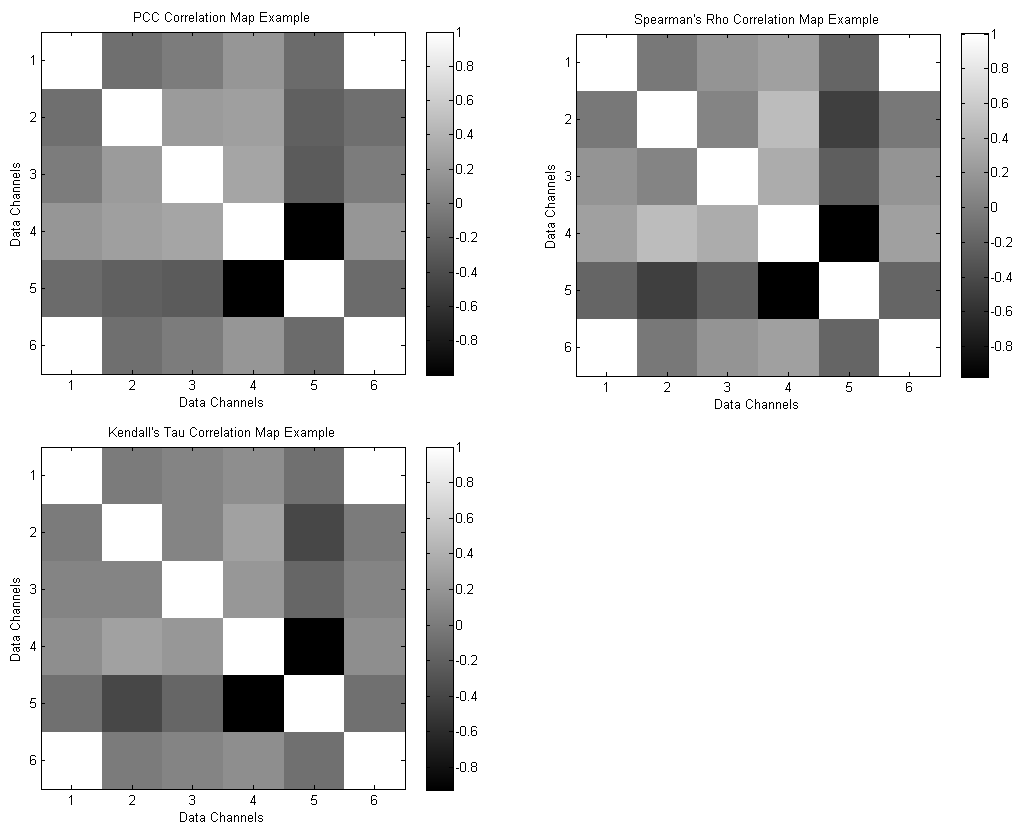
\includegraphics[width=\columnwidth]{images/correlation_comparison.png}
    \caption{Three common correlation coefficient algorithms are compared on a sample data set. Note that items 1 and 6 have a strong rank-based correlation, but the relationship is non-linear, resulting in a visibly lower correlation score within the PCC visualization. Also note the strong negative correlation between items 4 and 5.}
    \label{fig:correlation_comparison}
\end{figure}

\section{Animated Corrgrams}

Animated corrgrams are a potential solution to address the traditional corrgram's inability to capture changing correlative state over time. In an animated corrgram, the correlative state of a system is calculated over a retrospective time window, and every time new data is received, the correlative state is recalculated and redisplayed. The next chapter will walk through the creation of an animated corrgram with real system data. We have been unable to find any examples of animated corrgrams used in previous research for displaying changing system state over time.